\chapter{构建阀体三维模型}

{\bfseries 学习目标}
\begin{itemize}
\item 学习利用chamfer命令绘制图形
\item 学习利用chamferedge命令建立三维倒角
\end{itemize}

{\bfseries 任务要求}
\begin{itemize}
\item 根据图\ref{fig:tiaoyafafati}所示的杯零件图,用旋转法建立调压阀阀体零件的三维模型
\end{itemize}

\noindent
\begin{figure}[htbp]
\centering
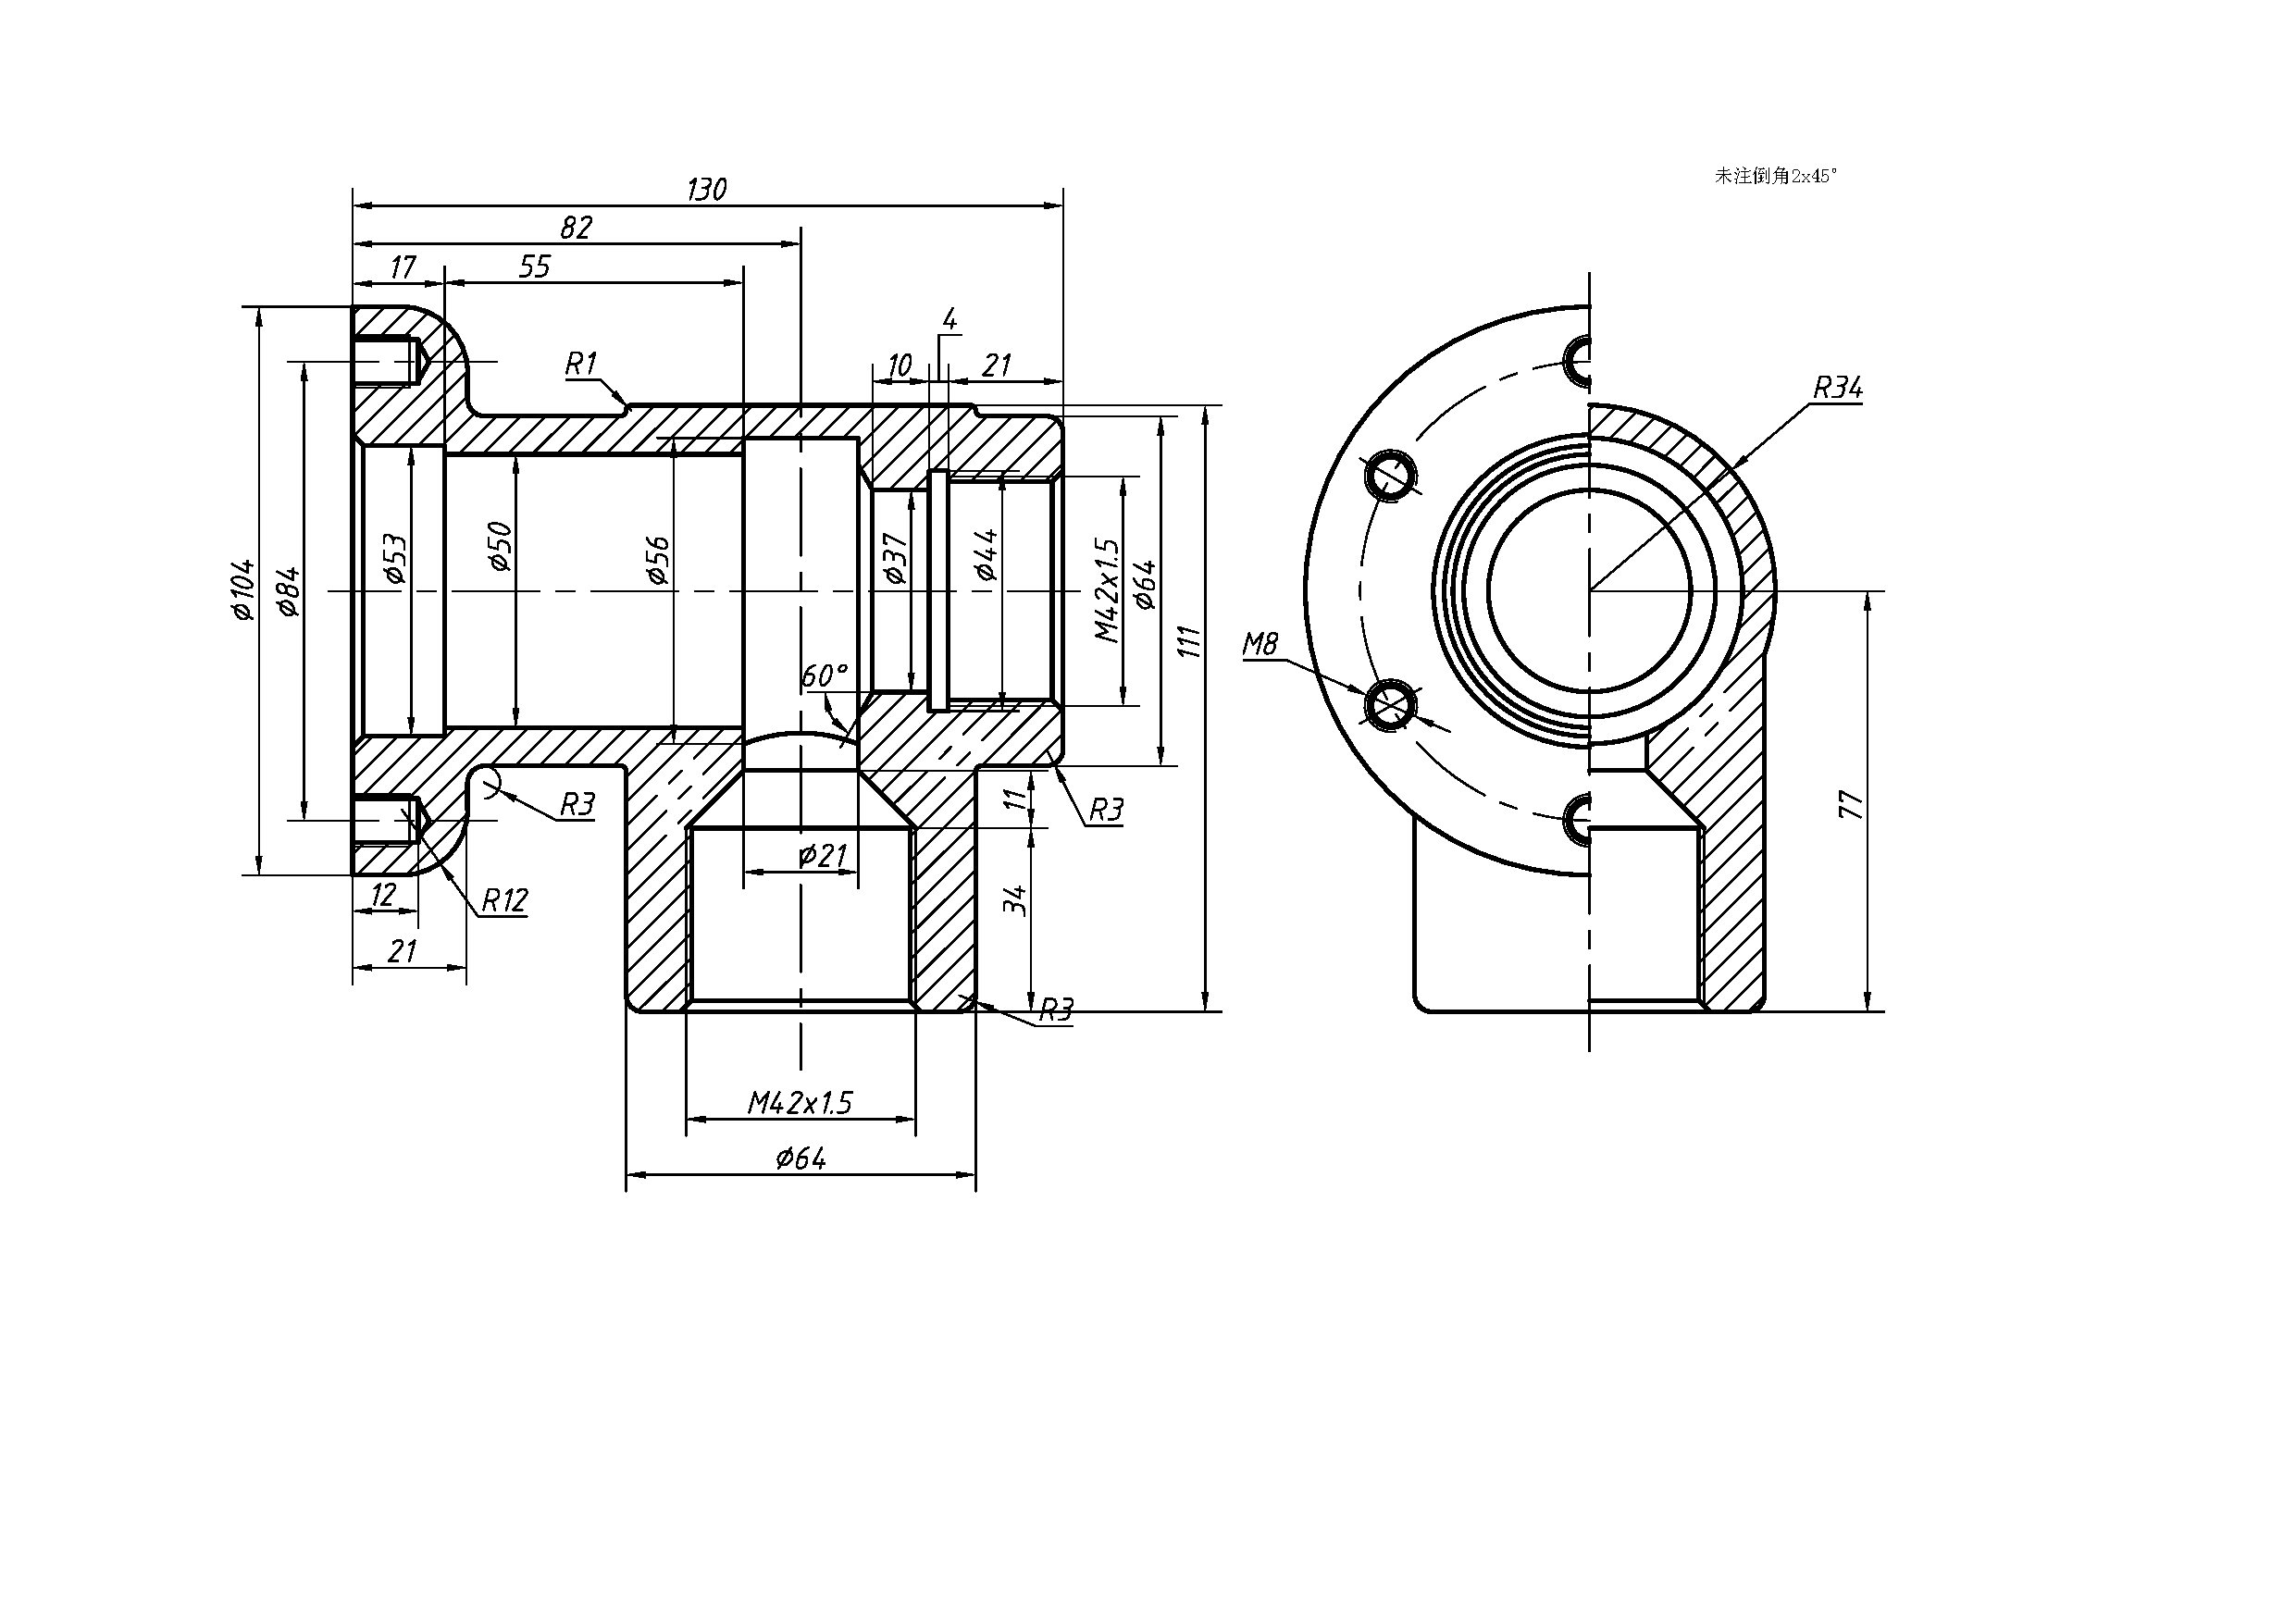
\includegraphics[scale=0.45]{tiaoyafafati.pdf}
\caption{阀体零件图}\label{fig:tiaoyafafati}
\end{figure}
\clearpage
\section{看组合体视图}
\subsection{识读要点}
\subsubsection{视图中线框和图形的理解}
一、视图中的每个线框,通常表示的是物体上一个表面(平面、曲面或平面和曲面相切)的投影。图\ref{fig:kantu8}中,线框A和E代表一个平面,线框F代表一个曲面,线框E代表平面和典相切。

二、视图中的相邻线框,表示物体上不同位置的两个表面。两个表面或是上下、左右、前后的位置关系,或者是两表面相交。图\ref{fig:kantu8}中,A、D两个面,A面在上,B面在下;A、D两个面,A面在右,D面在左。

\begin{figure}[htbp]
\centering
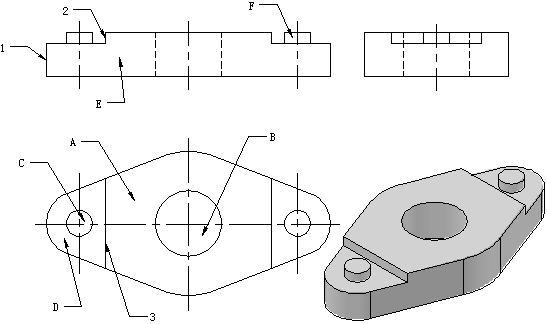
\includegraphics[scale=0.9]{kantu8.png}
\caption{线框和图形的含义}\label{fig:kantu8}
\end{figure}


三、视图中大线框套小线框,表示物体龙须面上凸出或凹进的关系。图\ref{fig:kantu8}中,C、D两个面,C为凸出;A、B两个面,B为凹进。

四、视图中的第一条线,可能是立体表面有积聚性表面的投影,如图\ref{fig:kantu8}中的线2;也可能是两平面的投影,如图\ref{fig:kantu8}中的线3;也可能是曲面转向轮廓线的投影,如图\ref{fig:kantu8}中的线1。
\subsubsection{联系多个视图进行识读}
在缺少尺寸瓢的情况下,一个视图是不能够确定物体的形状的。因为一个视图只能够表达两个方向的尺寸,一般不能够确切地表达出物体的三维空间形状。如图\ref{fig:kantu9}所示,如果仅仅只用主视图难以准确表达出物体的三维形状。根据俯视图的不同,物体的底板可能是倒角、凸字形和凹字形。因此,看图不能仅看一个或两个视图,而要把三个视图联系起来进行分析,才能够确定物体的形状。

\begin{figure}[htbp]
\centering
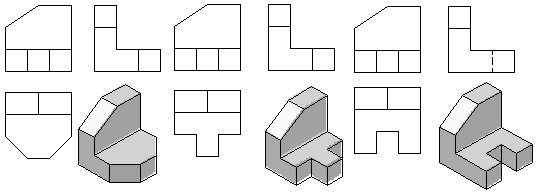
\includegraphics[scale=0.9]{kantu9.png}
\caption{一个视图不能确切地表达物体的形状}\label{fig:kantu9}
\end{figure}

如果视图选择不当,即使有两个视图也不能够准确地表达出物体的三维形状。如图\ref{fig:kantu9}所示,如果采用主视图和左视图就不能够清楚地表达出物体的形状。


\subsubsection{确定主特征视图}
特征视图是能够充分反映物体形状或相互位置特征的视图。特征视图通常分类形状特征视图和位置特征视图。形状特征图是能够充分反映物体形状特征的视图。图\ref{fig:kantu10}的主视图为形状特征视图,\ref{fig:kantu11}的俯视图为形状特征视图,它们都充分反映了特征的形状特征
\begin{figure}[htbp]
\centering
\subfloat[主视图为形状特征视图]{\label{fig:kantu10}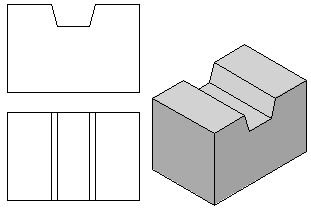
\includegraphics[scale=0.7]{kantu10.png}}\hspace{30pt}
\subfloat[俯视图为形状特征视图]{\label{fig:kantu11}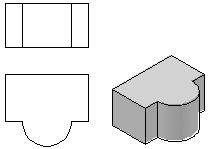
\includegraphics[scale=1]{kantu11.png}}
\caption{形状特征视图}
\end{figure}

位置特征图是能够充分反映相互位置特征的视图。图\ref{fig:kantu12}和\ref{fig:kantu13}所示的主视图是物体的形状特征图,但仅依靠主视图和俯视图不能够确定出1和2两个线框所代表的形状的具体位置。它们的左视图则清楚地反映方孔和圆柱的具体位置关系。
\begin{figure}[htbp]
\centering
\subfloat[]{\label{fig:kantu12}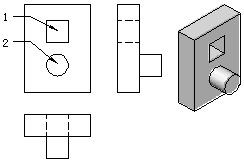
\includegraphics[scale=0.9]{kantu12.png}}\hspace{30pt}
\subfloat[]{\label{fig:kantu13}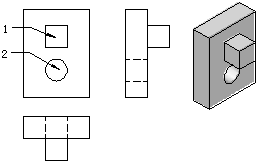
\includegraphics[scale=0.9]{kantu13.png}}
\caption{位置特征视图}
\end{figure}
\subsubsection{注意反映形体联接关系的图线}
形体之间的联接关系的变化,会导致视图中的图线产生相应的变化。图\ref{fig:kantu14}所示,三角形肋板与底板的连接是实线,说明它们的前面不是位于同一平面的错位关系,由俯视图可知三角形肋板位于底板中间。图\ref{fig:fati15}的中间是虚线连接,三角形肋板与底板的前面是位于同一个平面的,根据俯视图可以确定三角形肋板有两块,一块位于前面,另一块位于后面。
\begin{figure}[htbp]
\centering
\subfloat[]{\label{fig:kantu14}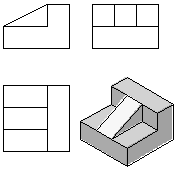
\includegraphics[scale=0.9]{kantu14.png}}\hspace{30pt}
\subfloat[]{\label{fig:kantu15}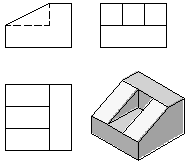
\includegraphics[scale=0.9]{kantu15.png}}
\caption{形体之间的表面联接关系}
\end{figure}
\endinput
\subsection{形体分析法}
形体分析法是从能够反映物体形状特征的视图出发,分析该物体由哪几个部分组成,采用什么形式组合,然后运用视图投影规律,找出每个部分在其它视图上的投影,从而想象出各个部分所表达的基本形体的形状及各部分之间的相互位置关系,最后综合想象出整个物体的形状的方法。

下面以图所示的三视图来说明形体分析法看图的步骤。

一、看视图,分析物体的形体组成部分。运用形体分析法将视图分成3个部分,如图\ref{fig:kantu}所示。
\begin{figure}[htbp]
\centering
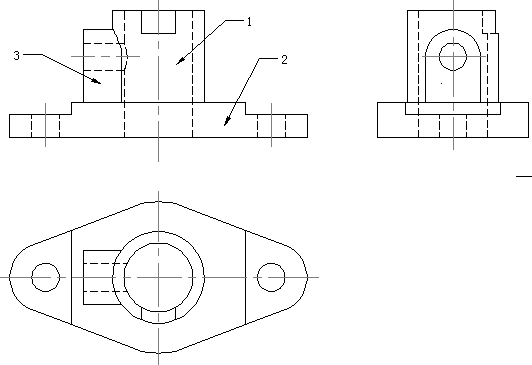
\includegraphics[scale=0.5]{kantu.png}
\caption{分析组成部分}\label{fig:kantu}
\end{figure}

二、找投影关系,想形体。从线框出发,从三视图中找出各个部分的投影,确定特征视图,想象形状。
\begin{figure}[htbp]
\centering
\subfloat[]{\label{fig:kantu3}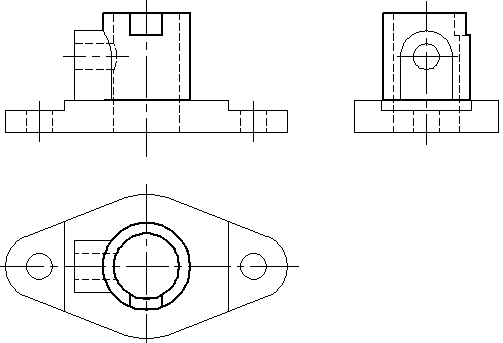
\includegraphics[scale=0.4]{kantu3.png}}\hspace{30pt}
\subfloat[]{\label{fig:kantu4}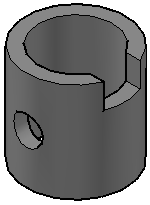
\includegraphics[scale=0.6]{kantu4.png}}
\caption{套筒部分}
\end{figure}

\begin{figure}[htbp]
\centering
\subfloat[]{\label{fig:kantu1}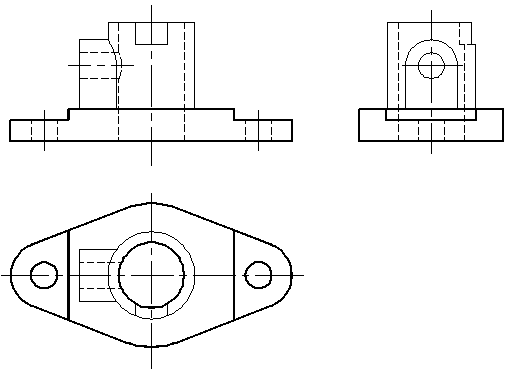
\includegraphics[scale=0.4]{kantu1.png}}\hspace{30pt}
\subfloat[]{\label{fig:kantu2}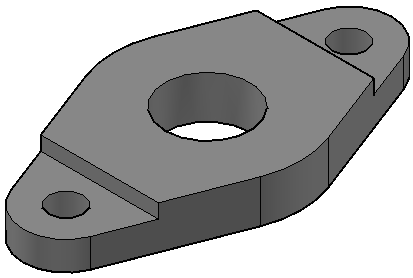
\includegraphics[scale=0.3]{kantu2.png}}
\caption{底板部分}
\end{figure}
图\ref{fig:kantu3}所示,粗实线为第1部分套筒的三视图,从三视图可知,该套筒上前部分开有缺口,左中部分开有孔,如图\ref{fig:kantu4}所示。

图\ref{fig:kantu1}所示,粗实线为第2部分底板的三视图,从三视图可知,该底板整体上为一凸台,并有三个通孔,如图\ref{fig:kantu2}所示。

图\ref{fig:kantu5}所示,粗实线为第三部分凸台的三视图,从三视可知,该凸台由四棱体和半圆柱构成,并且右边被圆柱曲面切割,上半部分有一通孔, 如图\ref{fig:kantu6}所示。

\begin{figure}[htbp]
\centering
\subfloat[]{\label{fig:kantu5}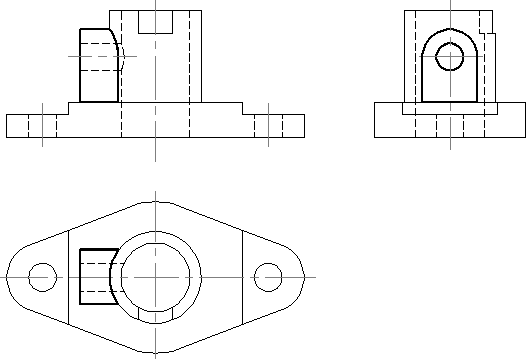
\includegraphics[scale=0.4]{kantu5.png}}\hspace{30pt}
\subfloat[]{\label{fig:kantu6}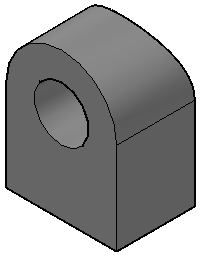
\includegraphics[scale=0.3]{kantu6.png}}
\caption{凸台部分}
\end{figure}

三、明确位置和连接关系。在想象出各部分形体后,需要利用位置特征视图,确定各部分的位置和表面连接关系。确定位置关系和表面连接关系通常是难以截然分开的,需要进行综合考虑。图\ref{fig:kantu}所示,第1部分位于第2部分上面正中心位置,第3部分位于第2部分上面,位于第1部分左边并与之相贯。

四、综合分析,想象整体。将上面各个部分的形体和位置分析综合起,便可以想角出整个形体,如图\ref{fig:kantu7}所示。
\begin{figure}[htbp]
\centering
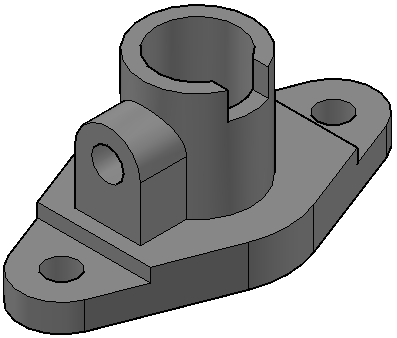
\includegraphics[scale=1]{kantu7.png}
\caption{支座空间形体}\label{fig:kantu7}
\end{figure}
\endinput
%\subsection{线面分析法}
线面分析法是分析组合体视图中某些线、面的投影关系,运用线、面的投影特征,分析视图中每一条线或线框所代表的含义和位置关系,用以确定物体形状的方法。

下面以为例来说明线面分析法看图的基本步骤。


\endinput
\section{构建阀体三维模型}
\section{构建阀体三维模型}
\subsection{绘制阀体旋转矩形}
\begin{procedure}
\item 设置图层。

建立“中心线”和“实线”两个图层,并将当前图层设置为“中心线”图层。
\item 切换视图方向为主视图方向。
\item 绘制辅助定位线,其结果如图\ref{fig:faticenterline}所示。
绘制阀体主对称中心线。
\begin{lstlisting}
|命令: XLINE|
|指定点或 [水平(H)/垂直(V)/角度(A)/二等分(B)/偏移(O)]: 82,77|
|指定通过点:$ @1<0$|
|指定通过点:$ @1<90$|
|指定通过点:|
\end{lstlisting}
偏移产生$M8$孔中心线。
\begin{lstlisting}
|命令: OFFSET|
|当前设置: 删除源=否  图层=源  OFFSETGAPTYPE=0|
|指定偏移距离或 [通过(T)/删除(E)/图层(L)]$<$通过$>$:  42|
|选择要偏移的对象,或 [退出(E)/放弃(U)] $<$退出$>$:|
|指定要偏移的那一侧上的点,或 [退出(E)/多个(M)/放弃(U)] $<$退出$>$:|
|选择要偏移的对象,或 [退出(E)/放弃(U)] $<$退出$>$:|
\end{lstlisting}
\begin{figure}[htbp]
\centering
\subfloat[]{\label{fig:faticenterline}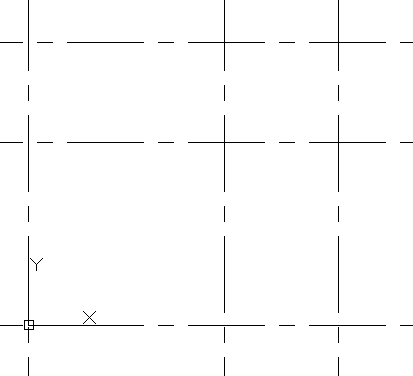
\includegraphics[scale=0.3]{faticenterline.png}}\hspace{30pt}
\subfloat[]{\label{fig:fati1}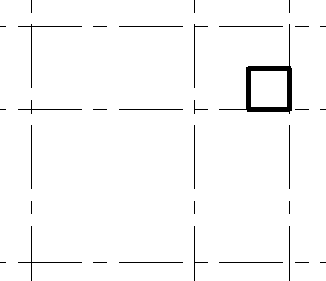
\includegraphics[scale=0.4]{fati1.png}}
\hspace{30pt}
\subfloat[]{\label{fig:fati2}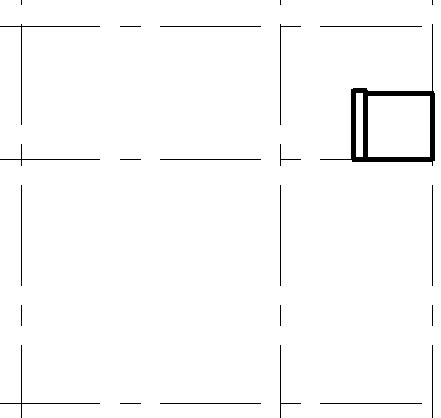
\includegraphics[scale=0.25]{fati2.png}}
\caption{旋转矩形绘制过程一}
\end{figure}
\item 切换图层为实线层,绘制端面定位线。
偏移生成左端面定位线。
\begin{lstlisting}
|命令: OFFSET|
|当前设置: 删除源=否  图层=源  OFFSETGAPTYPE=0|
|指定偏移距离或 [通过(T)/删除(E)/图层(L)]$<$42.0000$>$: 82|
|选择要偏移的对象,或 [退出(E)/放弃(U)] $<$退出$>$:|
|指定要偏移的那一侧上的点,或 [退出(E)/多个(M)/放弃(U)] $<$退出$>$:|
|选择要偏移的对象,或 [退出(E)/放弃(U)] $<$退出$>$:|
\end{lstlisting}
偏移产生右端面定位线。
\begin{lstlisting}
|命令: OFFSET|
|当前设置: 删除源=否  图层=源  OFFSETGAPTYPE=0|
|指定偏移距离或 [通过(T)/删除(E)/图层(L)]$<$82.0000$>$: 48|
|选择要偏移的对象,或 [退出(E)/放弃(U)] $<$退出$>$:|
|指定要偏移的那一侧上的点,或 [退出(E)/多个(M)/放弃(U)] $<$退出$>$:|
|选择要偏移的对象,或 [退出(E)/放弃(U)] $<$退出$>$:|
\end{lstlisting}
偏移产生下端面定位线。
\begin{lstlisting}
|命令: OFFSET|
|当前设置: 删除源=否  图层=源  OFFSETGAPTYPE=0|
|指定偏移距离或 [通过(T)/删除(E)/图层(L)]$<$48.0000$>$: 77|
|选择要偏移的对象,或 [退出(E)/放弃(U)] $<$退出$>$:|
|指定要偏移的那一侧上的点,或 [退出(E)/多个(M)/放弃(U)] $<$退出$>$:|
|选择要偏移的对象,或 [退出(E)/放弃(U)] $<$退出$>$:|
\end{lstlisting}
\item 绘制孔旋转矩形

绘制$M42$水平螺孔旋转矩形,如图\ref{fig:fati1}所示。
\begin{lstlisting}
|命令:  RECTANG|
|指定第一个角点或 [倒角(C)/标高(E)/圆角(F)/厚度(T)/|
|宽度(W)]: int 于|
|指定另一个角点或 [面积(A)/尺寸(D)/旋转(R)]: @-21,21|
\end{lstlisting}
绘制$\phi 44$孔旋转矩形,如图\ref{fig:fati2}所示。
\begin{lstlisting}
|命令:  RECTANG|
|指定第一个角点或 [倒角(C)/标高(E)/圆角(F)/厚度(T)/|
|宽度(W)]: int 于|
|指定另一个角点或 [面积(A)/尺寸(D)/旋转(R)]: @-4,22|
\end{lstlisting}
\begin{figure}[htbp]
\centering
\subfloat[]{\label{fig:fati3}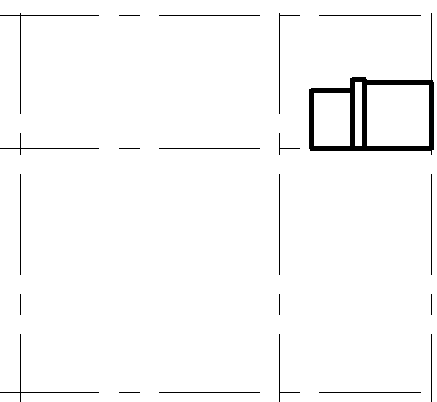
\includegraphics[scale=0.32]{fati3.png}}\hspace{30pt}
\subfloat[]{\label{fig:fati4}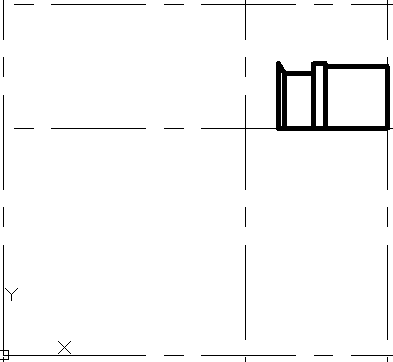
\includegraphics[scale=0.35]{fati4.png}}
\hspace{30pt}
\subfloat[]{\label{fig:fati5}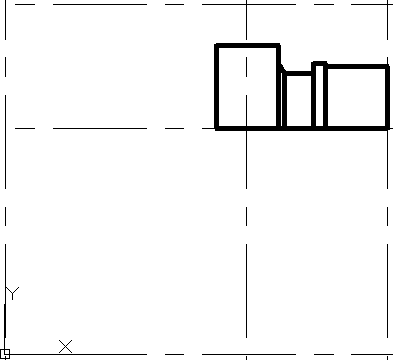
\includegraphics[scale=0.35]{fati5.png}}
\caption{旋转矩形绘制过程二}
\end{figure}
绘制$\phi 37$孔旋转矩形,如图\ref{fig:fati3}所示。
\begin{lstlisting}
|命令:  RECTANG|
|指定第一个角点或 [倒角(C)/标高(E)/圆角(F)/厚度(T)/|
|宽度(W)]: int 于|
|指定另一个角点或 [面积(A)/尺寸(D)/旋转(R)]: @-10,18.5|
\end{lstlisting}
绘制$2X45^o$倒角孔旋转梯形,其结果如图\ref{fig:fati4}所示。
\begin{lstlisting}
|命令: line|
|指定第一个点:int 于|
|指定下一点或 [放弃(U)]:end 于|
|指定下一点或 [放弃(U)]: @4<120|
|指定下一点或 [闭合(C)/放弃(U)]:per 于|
|指定下一点或 [闭合(C)/放弃(U)]:c|
\end{lstlisting}
面域$2X45^o$倒角孔旋转梯形。
\begin{lstlisting}
|命令: REGION|
|选择对象: 找到 1 个|
|选择对象: 找到 1 个,总计 2 个|
|选择对象: 找到 1 个,总计 3 个|
|选择对象: 找到 1 个,总计 4 个|
|选择对象:|
|已提取 1 个环。|
|已创建 1 个面域。|
\end{lstlisting}
绘制$\phi 56$孔旋转矩形,如图\ref{fig:fati5}所示。
\begin{lstlisting}
|命令:  RECTANG|
|指定第一个角点或 [倒角(C)/标高(E)/圆角(F)/厚度(T)/|
|宽度(W)]: int 于|
|指定另一个角点或 [面积(A)/尺寸(D)/旋转(R)]: @-21,28|
\end{lstlisting}
绘制$\phi 56$孔旋转矩形,如图\ref{fig:fati6}所示。
\begin{lstlisting}
|命令:  RECTANG|
|指定第一个角点或 [倒角(C)/标高(E)/圆角(F)/厚度(T)/|
|宽度(W)]: int 于|
|指定另一个角点或 [面积(A)/尺寸(D)/旋转(R)]: @-55,25|
\end{lstlisting}
绘制$\phi 53$孔旋转矩形,如图\ref{fig:fati7}所示。
\begin{lstlisting}
|命令:  RECTANG|
|指定第一个角点或 [倒角(C)/标高(E)/圆角(F)/厚度(T)/|
|宽度(W)]: int 于|
|指定另一个角点或 [面积(A)/尺寸(D)/旋转(R)]: @-17,26.5|
\end{lstlisting}
\begin{figure}[htbp]
\centering
\subfloat[]{\label{fig:fati6}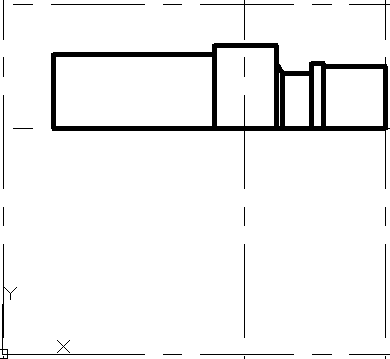
\includegraphics[scale=0.3]{fati6.png}}\hspace{30pt}
\subfloat[]{\label{fig:fati7}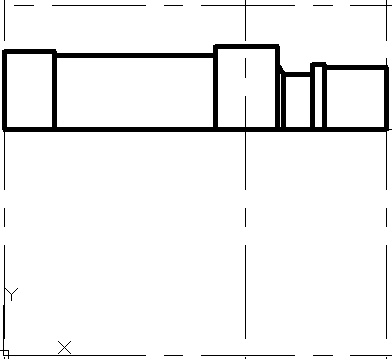
\includegraphics[scale=0.3]{fati7.png}}\\
\subfloat[]{\label{fig:fati8}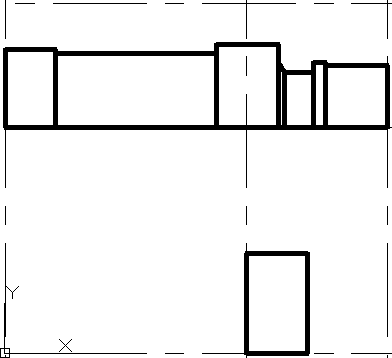
\includegraphics[scale=0.3]{fati8.png}}\hspace{30pt}
\subfloat[]{\label{fig:fati9}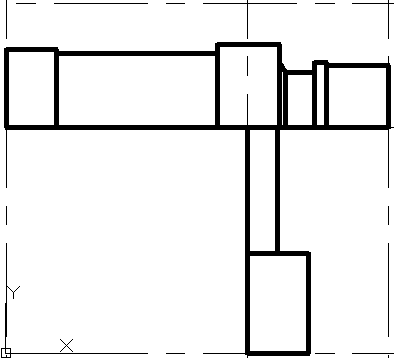
\includegraphics[scale=0.3]{fati9.png}}
\caption{旋转矩形绘制过程三}
\end{figure}
绘制$M42$垂直螺孔旋转矩形,如图\ref{fig:fati8}所示。
\begin{lstlisting}
|命令:  RECTANG|
|指定第一个角点或 [倒角(C)/标高(E)/圆角(F)/厚度(T)/|
|宽度(W)]: int 于|
|指定另一个角点或 [面积(A)/尺寸(D)/旋转(R)]: @21,34|
\end{lstlisting}
绘制$\phi 21$孔旋转矩形,如图\ref{fig:fati9}所示。
\begin{lstlisting}
|命令:  RECTANG|
|指定第一个角点或 [倒角(C)/标高(E)/圆角(F)/厚度(T)/|
|宽度(W)]: int 于|
|指定另一个角点或 [面积(A)/尺寸(D)/旋转(R)]: @10.5,43|
\end{lstlisting}
绘制$M8$孔旋转矩形,如图\ref{fig:fati10}所示。
\begin{lstlisting}
|命令:  RECTANG|
|指定第一个角点或 [倒角(C)/标高(E)/圆角(F)/厚度(T)/|
|宽度(W)]: int 于|
|指定另一个角点或 [面积(A)/尺寸(D)/旋转(R)]: @14,4|
\end{lstlisting}
\begin{figure}[htbp]
\centering
\subfloat[]{\label{fig:fati10}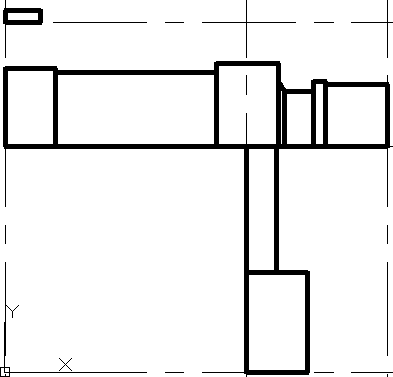
\includegraphics[scale=0.38]{fati10.png}}\hspace{30pt}
\subfloat[]{\label{fig:fati11}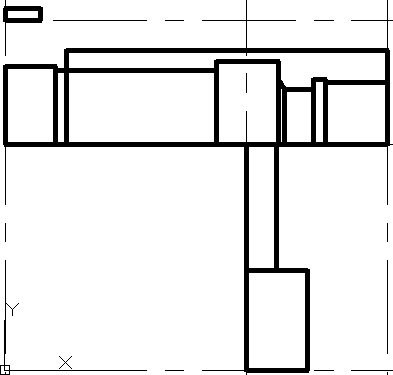
\includegraphics[scale=0.38]{fati11.png}}\\
\subfloat[]{\label{fig:fati12}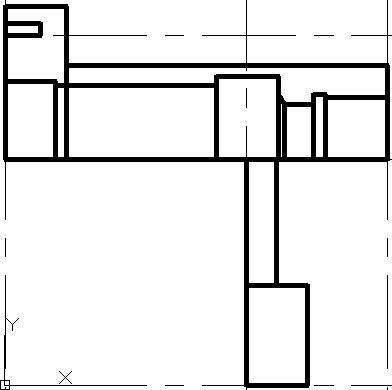
\includegraphics[scale=0.38]{fati12.png}}\hspace{30pt}
\subfloat[]{\label{fig:fati13}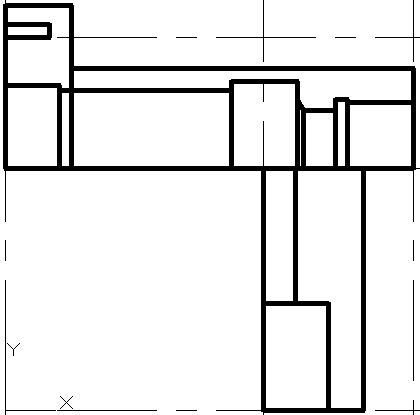
\includegraphics[scale=0.35]{fati13.png}}
\caption{旋转矩形绘制过程四}
\end{figure}
\item 绘制阀体旋转矩形

绘制$\phi 64$水平圆柱旋转矩形,结果如图\ref{fig:fati11}所示。
\begin{lstlisting}
|命令:  RECTANG|
|指定第一个角点或 [倒角(C)/标高(E)/圆角(F)/厚度(T)/|
|宽度(W)]: int 于|
|指定另一个角点或 [面积(A)/尺寸(D)/旋转(R)]: @-109,32|
\end{lstlisting}
绘制$\phi 104$圆柱旋转矩形,结果如图\ref{fig:fati12}所示。
\begin{lstlisting}
|命令:  RECTANG|
|指定第一个角点或 [倒角(C)/标高(E)/圆角(F)/厚度(T)/|
|宽度(W)]: int 于|
|指定另一个角点或 [面积(A)/尺寸(D)/旋转(R)]: @21,52|
\end{lstlisting}
绘制$\phi 64$垂直圆柱旋转矩形,结果如图\ref{fig:fati13}所示。
\begin{lstlisting}
|命令:  RECTANG|
|指定第一个角点或 [倒角(C)/标高(E)/圆角(F)/厚度(T)/|
|宽度(W)]: int 于|
|指定另一个角点或 [面积(A)/尺寸(D)/旋转(R)]: @32,77|
\end{lstlisting}
绘制$R34$水平圆柱旋转矩形,结果如图 所示。
\begin{lstlisting}
|命令: RECTANG|
|指定第一个角点或 [倒角(C)/标高(E)/圆角(F)/厚度(T)|
|/宽度(W)]: 50,77|
|指定另一个角点或 [面积(A)/尺寸(D)/旋转(R)]: @64,34|
\end{lstlisting}
绘制$M8$螺孔倒角,其结果如图 所示。倒角命令的启动方法有:
\begin{itemize}
\item 键盘输入CHAMFER或CHA。
\item 点击【修改】菜单中【倒角】项。
\item 点击【修改】工具栏中的【倒角】图标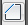
\includegraphics[scale=0.6]{chamfer.png}
\end{itemize}
\begin{lstlisting}
|命令: CHAMFER|
|(“修剪”模式) 当前倒角距离 1 = 0.0000,距离 2 = 0.0000|
|选择第一条直线或 [放弃(U)/多段线(P)/距离(D)/角度(A)/修剪(T)|
|/方式(E)/多个(M)]:  d |
|指定 第一个 倒角距离 $<$0.0000$>$: 2 |
|指定 第二个 倒角距离 $<$2.0000$>$: 4|
|选择第一条直线或 [放弃(U)/多段线(P)/距离(D)/角度(A)/修剪(T)|
|/方式(E)/多个(M)]:|
|选择第二条直线,或按住 Shift 键选择直线以应用角点或 [距离(D)|
|/角度(A)/方法(M)]:|
\end{lstlisting}
\begin{figure}[htbp]
\centering
\subfloat[]{\label{fig:fati14}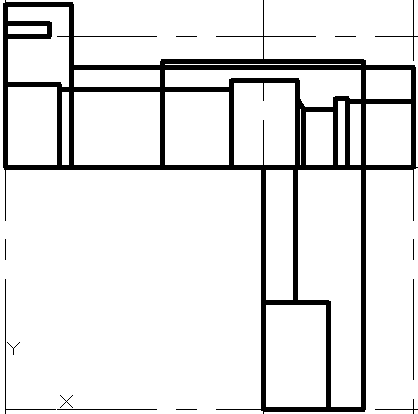
\includegraphics[scale=0.38]{fati14.png}}\hspace{30pt}
\subfloat[]{\label{fig:fati15}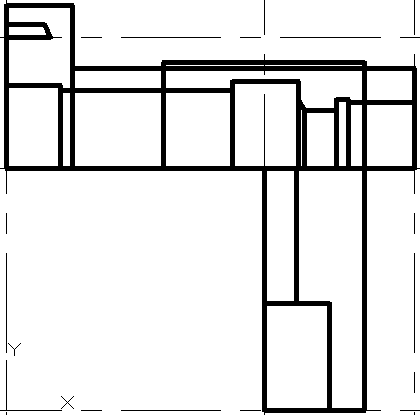
\includegraphics[scale=0.38]{fati15.png}}
\caption{旋转矩形绘制过程五}
\end{figure}

\end{procedure}
\endinput

\subsection{构建阀体三维模型}
\begin{procedure}
\item 切换视图方向为西南等轴测。
\item 旋转产生孔实体。

旋转产生水平孔实体,其结果如图\ref{fig:fatisolid1} 所示。
\begin{lstlisting}
|命令: REVOLVE|
|当前线框密度:  ISOLINES=4,闭合轮廓创建模式 = 实体|
|选择要旋转的对象或 [模式(MO)]: 找到 1 个|
|选择要旋转的对象或 [模式(MO)]: 找到 1 个,总计 2 个|
|选择要旋转的对象或 [模式(MO)]: 找到 1 个,总计 3 个|
|选择要旋转的对象或 [模式(MO)]: 找到 1 个,总计 4 个|
|选择要旋转的对象或 [模式(MO)]: 找到 1 个,总计 5 个|
|选择要旋转的对象或 [模式(MO)]: 找到 1 个,总计 6 个|
|选择要旋转的对象或 [模式(MO)]: 找到 1 个,总计 7 个|
|选择要旋转的对象或 [模式(MO)]:|
|指定轴起点或根据以下选项之一定义轴 [对象(O)/X/Y/Z] $<$对象$>$:|
|指定轴端点:|
|指定旋转角度或 [起点角度(ST)/反转(R)/表达式(EX)] $<$360$>$:|
\end{lstlisting}
\begin{figure}[htbp]
\centering
\subfloat[]{\label{fig:fatisolid1}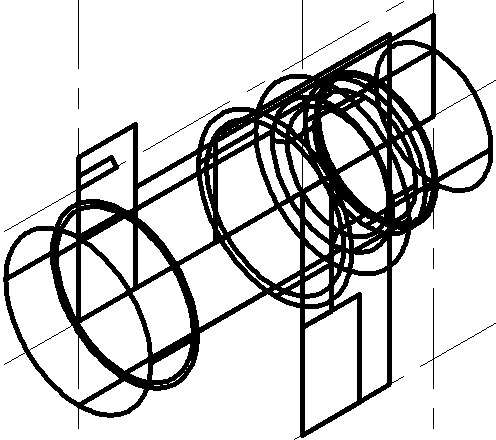
\includegraphics[scale=0.31]{fatisolid1.png}}\hspace{30pt}
\subfloat[]{\label{fig:fatisolid2}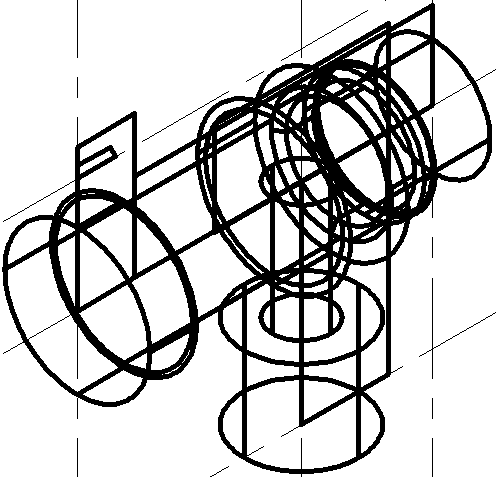
\includegraphics[scale=0.31]{fatisolid2.png}}\\
\subfloat[]{\label{fig:fatisolid3}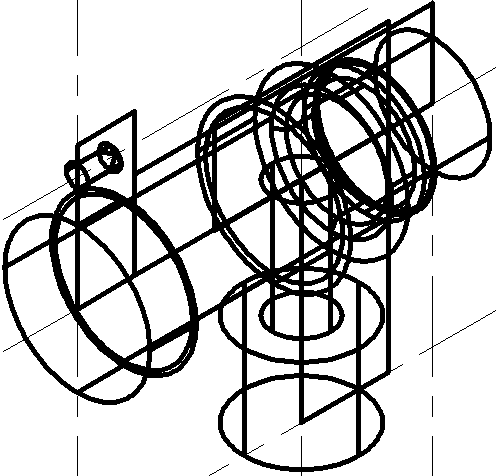
\includegraphics[scale=0.31]{fatisolid3.png}}\hspace{30pt}
\subfloat[]{\label{fig:fatisolid4}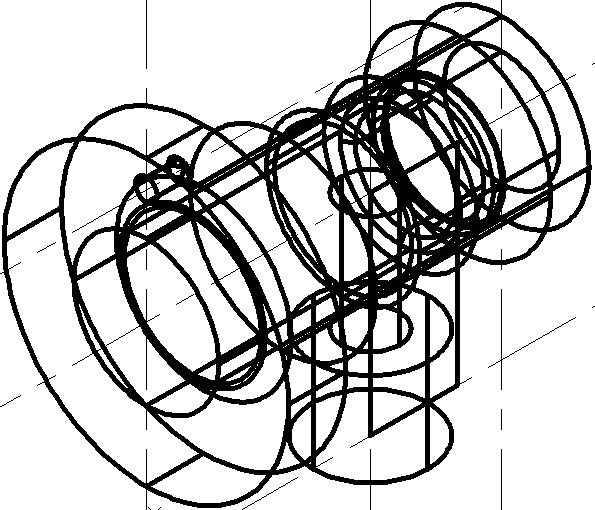
\includegraphics[scale=0.3]{fatisolid4.png}}
\caption{阀体三维模型构建过程一}
\end{figure}
旋转产生垂直孔实体,其结果如图\ref{fig:fatisolid2}所示。
\begin{lstlisting}
|命令: REVOLVE|
|当前线框密度:  ISOLINES=4,闭合轮廓创建模式 = 实体|
|选择要旋转的对象或 [模式(MO)]: 找到 1 个|
|选择要旋转的对象或 [模式(MO)]: 找到 1 个,总计 2 个|
|选择要旋转的对象或 [模式(MO)]:|
|指定轴起点或根据以下选项之一定义轴 [对象(O)/X/Y/Z] $<$对象$>$:|
|指定轴端点:|
|指定旋转角度或 [起点角度(ST)/反转(R)/表达式(EX)] $<$360$>$:|
\end{lstlisting}
旋转产生$M8$螺孔实体,其结果如图\ref{fig:fatisolid3}所示。
\begin{lstlisting}
|命令: REVOLVE|
|当前线框密度:  ISOLINES=4,闭合轮廓创建模式 = 实体|
|选择要旋转的对象或 [模式(MO)]: 找到 1 个|
|选择要旋转的对象或 [模式(MO)]:|
|指定轴起点或根据以下选项之一定义轴 [对象(O)/X/Y/Z] $<$对象$>$:|
|指定轴端点:|
|指定旋转角度或 [起点角度(ST)/反转(R)/表达式(EX)] $<$360$>$:|
\end{lstlisting}
旋转产生水平阀体实体,其结果如图\ref{fig:fatisolid4}所示。
\begin{lstlisting}
|命令: REVOLVE|
|当前线框密度:  ISOLINES=4,闭合轮廓创建模式 = 实体|
|选择要旋转的对象或 [模式(MO)]: 找到 1 个|
|选择要旋转的对象或 [模式(MO)]: 找到 1 个,总计 2 个|
|选择要旋转的对象或 [模式(MO)]:|
|指定轴起点或根据以下选项之一定义轴 [对象(O)/X/Y/Z] $<$对象$>$:|
|指定轴端点:|
|指定旋转角度或 [起点角度(ST)/反转(R)/表达式(EX)] $<$360$>$:|
\end{lstlisting}
\begin{figure}[htbp]
\centering
\subfloat[]{\label{fig:fatisolid5}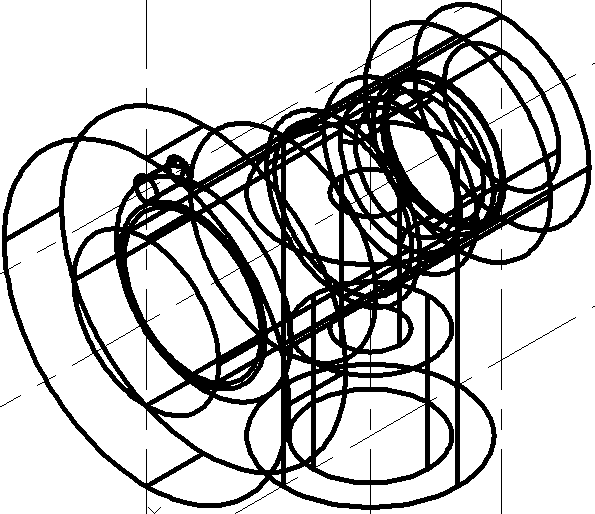
\includegraphics[scale=0.35]{fatisolid5.png}}\hspace{30pt}
\subfloat[]{\label{fig:fatisolid6}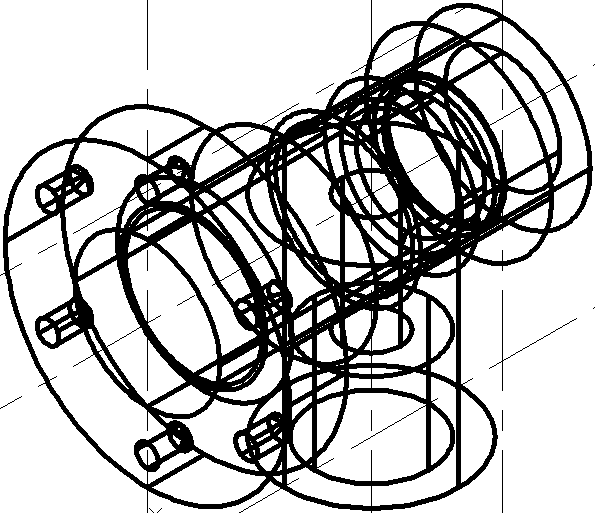
\includegraphics[scale=0.35]{fatisolid6.png}}\\
\subfloat[]{\label{fig:fatisolid7}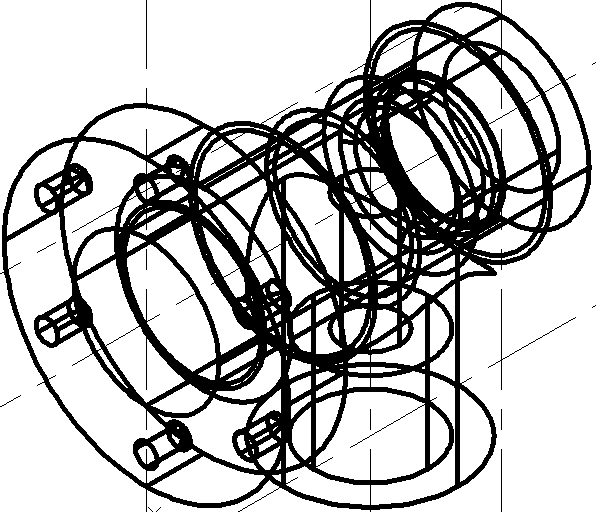
\includegraphics[scale=0.35]{fatisolid7.png}}\hspace{30pt}
\subfloat[]{\label{fig:fatisolid8}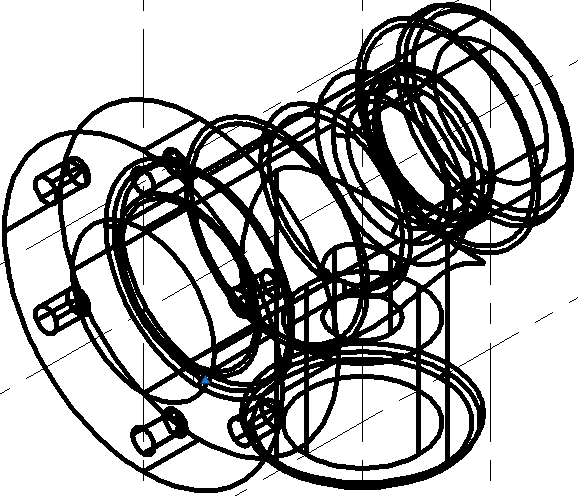
\includegraphics[scale=0.4]{fatisolid8.png}}
\caption{阀体三维模型构建过程二}
\end{figure}

旋转产生垂直阀体实体,其结果如图\ref{fig:fatisolid5}所示。
\begin{lstlisting}
|命令: REVOLVE|
|当前线框密度:  ISOLINES=4,闭合轮廓创建模式 = 实体|
|选择要旋转的对象或 [模式(MO)]: 找到 1 个|
|选择要旋转的对象或 [模式(MO)]:|
|指定轴起点或根据以下选项之一定义轴 [对象(O)/X/Y/Z] $<$对象$>$:|
|指定轴端点:|
|指定旋转角度或 [起点角度(ST)/反转(R)/表达式(EX)] $<$360$>$:|
\end{lstlisting}
\item 阵列生成6个$M8$螺孔,其结果如图\ref{fig:fatisolid6}。
\begin{lstlisting}
|命令: 3darray|
|选择对象: 找到 1 个|
|选择对象:|
|输入阵列类型 [矩形(R)/环形(P)]$<$矩形$>$:p|
|输入阵列中的项目数目: 6|
|指定要填充的角度 (+=逆时针, -=顺时针)$ <360>$:|
|旋转阵列对象? [是(Y)/否(N)] $<Y>$:|
|指定阵列的中心点:|
|指定旋转轴上的第二点:|
\end{lstlisting}
\item 合并阀实体。

将两个$\phi 64$圆柱体和$\phi 104$圆柱体合并为一个实体其结果如图\ref{fig:fatisolid7}所示。
\begin{lstlisting}
|命令: UNION|
|选择对象: 找到 1 个|
|选择对象: 找到 1 个,总计 2 个|
|选择对象: 找到 1 个,总计 3 个|
|选择对象:|
\end{lstlisting}

\item 生成阀体孔。
\begin{lstlisting}
|命令: SUBTRACT|
|选择要从中减去的实体、曲面和面域...|
|选择对象: 找到 1 个|
|选择对象:  选择要减去的实体、曲面和面域...|
|选择对象: 指定对角点: 找到 16 个|
|选择对象:|
\end{lstlisting}
\item 设置视觉样式为灰度,并将视图方向切换为东南等轴测。
\item 生成三维圆角

生成$R3$圆角,其结果如图\ref{fig:fatisolid8}所示。
\begin{lstlisting}
|命令: FILLETEDGE|
|半径 = 1.0000|
|选择边或 [链(C)/环(L)/半径(R)]: r|
|输入圆角半径或 [表达式(E)] $<$1.0000$>$: 3|
|选择边或 [链(C)/环(L)/半径(R)]:|
|选择边或 [链(C)/环(L)/半径(R)]:|
|选择边或 [链(C)/环(L)/半径(R)]:|
|选择边或 [链(C)/环(L)/半径(R)]:|
|已选定 3 个边用于圆角。|
|按 Enter 键接受圆角或 [半径(R)]:|
\end{lstlisting}
生成$R1$圆角。
\begin{lstlisting}
|命令: FILLETEDGE|
|半径 = 3.0000|
|选择边或 [链(C)/环(L)/半径(R)]: r|
|输入圆角半径或 [表达式(E)] $<$3.0000$>$: 1|
|选择边或 [链(C)/环(L)/半径(R)]:|
|选择边或 [链(C)/环(L)/半径(R)]:|
|选择边或 [链(C)/环(L)/半径(R)]:|
|已选定 2 个边用于圆角。|
|按 Enter 键接受圆角或 [半径(R)]:|
\end{lstlisting}
\item 生成三维倒角,其结果如图\ref{fig:fatisolid9}所示。

启动三维角命令的方法有:
\begin{itemize}
\item 键盘输入CHAMFEREDGE。
\item 点击【修改】中的【实体编辑】子菜单中的【倒角边】项。
\item 点击【实体编辑】工具栏中的【倒角边】图标
\includegraphics[scale=0.6]{chamferedge.png}。
\end{itemize}
生成$M42$水平螺孔倒角。
\begin{lstlisting}
|命令:CHAMFEREDGE|
|距离 1 = 2.0000,距离 2 = 4.0000|
|选择一条边或 [环(L)/距离(D)]: d|
|指定距离 1 或 [表达式(E)] $<$2.0000$>$:|
|指定距离 2 或 [表达式(E)] $<$4.0000$>$: 2|
|选择一条边或 [环(L)/距离(D)]:|
|选择同一个面上的其他边或 [环(L)/距离(D)]:|
|按 Enter 键接受倒角或 [距离(D)]:|
\end{lstlisting}
生成$M42$垂直螺孔倒角。
\begin{lstlisting}
|命令:  CHAMFEREDGE|
|距离 1 = 2.0000,距离 2 = 2.0000|
|选择一条边或 [环(L)/距离(D)]:|
|选择同一个面上的其他边或 [环(L)/距离(D)]:|
|按 Enter 键接受倒角或 [距离(D)]:|
\end{lstlisting}
生成$\phi 53$孔倒角。
\begin{lstlisting}
|命令:  CHAMFEREDGE|
|距离 1 = 2.0000,距离 2 = 2.0000|
|选择一条边或 [环(L)/距离(D)]:|
|选择同一个面上的其他边或 [环(L)/距离(D)]:|
|按 Enter 键接受倒角或 [距离(D)]:|
\end{lstlisting}
\begin{figure}[htbp]
\centering
\subfloat[]{\label{fig:fatisolid9}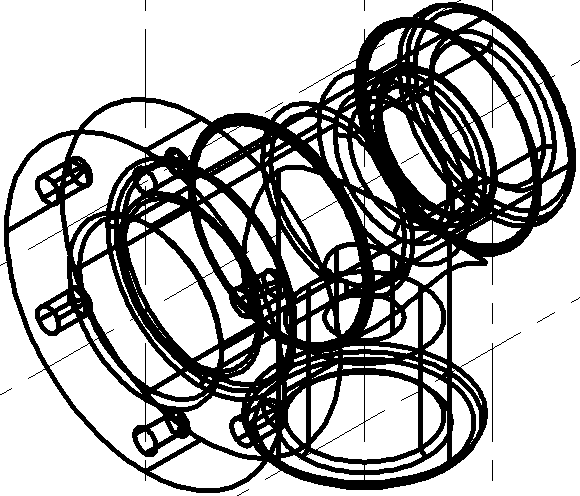
\includegraphics[scale=0.35]{fatisolid9.png}}\hspace{30pt}
\subfloat[]{\label{fig:fatisolid10}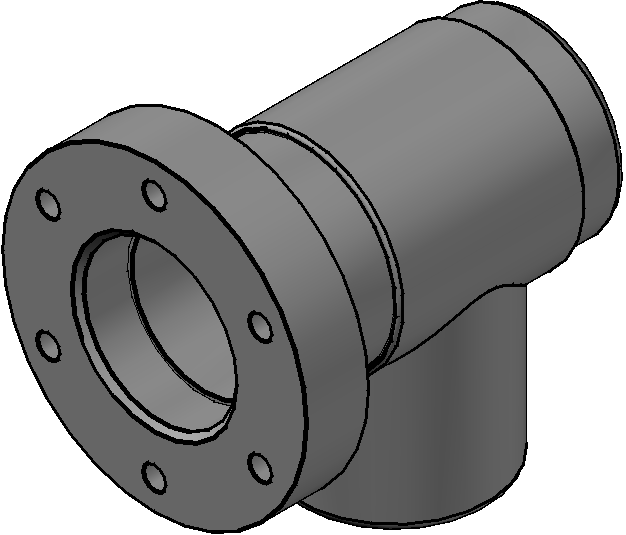
\includegraphics[scale=0.35]{fatisolid10.png}}
\caption{阀体三维模型构建过程三}
\end{figure}
\item 设置视觉样式为灰度,其结果如图\ref{fig:fatisolid10}所示。
\item 将端盖模型保存为“调压阀阀体立体图.dwg”。
\end{procedure}
\endinput
\endinput